\section{Results} \label{sec:results}
%One of the main contributions of this research is the proposal to use an alternative PRNG to the one used by Howe et al. \cite{howe2018standard}, cSHAKE. Comparatively, 
In this section we present the results obtained when implementing our FrodoKEM architecture. We provide a table of results for each of the key generation, encapsulation, and decapsulation designs in Tables \ref{tab:keyresults}, \ref{tab:encapsresults}, and \ref{tab:decapsresults}, respectively. We also provide results for the PRNG and Gaussian sampler in Table \ref{tab:otherresults}. All tables give comparative results of the previous FrodoKEM design in hardware, which utilize 1x LWE multiplier per clock cycle and completely conform to the FrodoKEM specifications by using cSHAKE where we are using Trivium. Moreover, all results are benchmarked on the same FPGA device as previous work, Xilinx Artix-7 XC7A35T FPGA, running on Vivado 2019.1.

\begin{table}
\centering
\caption{FPGA resource consumption of the proposed FrodoKEM \textbf{KeyGen} designs, using $k$ parallel multipliers, for both parameter sets, on a Xilinx Artix-7 FPGA.}\label{tab:keyresults}
%\vspace{-.2cm}
\resizebox{\columnwidth}{!}{

%\resizebox{0.7\textwidth}{!}{
%\noindent\makebox[\textwidth]{
\begin{tabular}{l r r r c c r}
\hline \Tstrut
  \textsc{FrodoKEM} & \multirow{2}{*}{LUT} & \multirow{2}{*}{FF} & \multirow{2}{*}{Slices} & DSP/ & \multirow{2}{*}{MHz} & Ops/ \\
Protocol &&&& BRAM && Sec  \\ \hline \Tstrut
%\textbf{} & & & \textbf{BRAM} & &\textbf{Sec} \\ \hline

KeyGen-640 1x & 971 & 433 & 290 & 1/0 & 191 & 59 \\
KeyGen-640 4x & 1174 & 781 & 355 & 4/0 & 185 & 226 \\
KeyGen-640 8x & 1679 & 1570 & 532 & 8/0 & 182 & 445 \\
KeyGen-640 16x & 2587 & 2994 & 855 & 16/0 & 172 & 840 \\ \hline \Tstrut
KeyGen-640 \cite{howe2018standard} & 3771 & 1800 & 1035 & 1/6 & 167 & 51 \\ \hline \Tstrut

KeyGen-976 1x & 1243 & 441 & 362 & 1/0 & 189 & 25 \\
KeyGen-976 4x & 1458 & 792 & 440 & 4/0 & 184 & 97 \\
KeyGen-976 8x & 1967 & 1576 & 617 & 8/0 & 178 & 187 \\
KeyGen-976 16x & 2869 & 3000 & 908 & 16/0 & 169 & 355 \\ \hline \Tstrut
KeyGen-976 \cite{howe2018standard} & 7139 & 1800 & 1939 & 1/8 & 167 & 22 \\ \hline \Tstrut

\end{tabular}}
\end{table}

\begin{table}
\centering
\caption{FPGA resource consumption of the proposed FrodoKEM \textbf{Encapsulation} designs, using $k$ parallel multipliers, for both parameter sets, on a Xilinx Artix-7 FPGA.}\label{tab:encapsresults}
%\vspace{-.2cm}
%\resizebox{0.7\textwidth}{!}{
%\noindent\makebox[\textwidth]{
\resizebox{\columnwidth}{!}{

\begin{tabular}{l r r r c c r}
\hline \Tstrut
  \textsc{FrodoKEM} & \multirow{2}{*}{LUT} & \multirow{2}{*}{FF} & \multirow{2}{*}{Slices} & DSP/ & \multirow{2}{*}{MHz} & Ops/ \\
Protocol &&&& BRAM && Sec  \\ \hline \Tstrut
%\textbf{} & & & \textbf{BRAM} & &\textbf{Sec} \\ \hline

Encaps-640 1x & 4246 & 2131 & 1180 & 1/0 & 190 & 58 \\
Encaps-640 4x & 4620 & 2552 & 1338 & 4/0 & 183 & 221 \\
Encaps-640 8x & 5155 & 3356 & 1485 & 8/0 & 177 & 427 \\
Encaps-640 16x & 5796 & 4694 & 1692 & 16/0 & 171 & 825 \\ \hline \Tstrut
Encaps-640 \cite{howe2018standard} & 6745 & 3528 & 1855 & 1/11 & 167 & 51 \\ \hline \Tstrut


Encaps-976 1x & 4650 & 2118 & 1272 & 1/0 & 187 & 25 \\
Encaps-976 4x & 4996 & 2611 & 1455 & 4/0 & 180 & 94 \\
Encaps-976 8x & 5562 & 3349 & 1608 & 8/0 & 175 & 183 \\
Encaps-976 16x & 6188 & 4678 & 1782 & 16/0 & 168 & 350 \\ \hline \Tstrut

Encaps-976 \cite{howe2018standard} & 7209 & 3537 & 1985 & 1/16 & 167 & 22 \\ \hline \Tstrut

\end{tabular}}
\end{table}


The first analysis is directed towards the performance of the PRNG. When compared to cSHAKE, the PRNG previously used in literature, Trivium (the PRNG we propose to use), occupies 4.5x less area on the FPGA (measured in slices). This means that when we instantiate a higher number of parallel multipliers, we consume far less FPGA area than what would be needed when using cSHAKE, as discussed in the algorithm proposal. The increase in area occupation, due to parallelising, is essentially the only reason for area increase when we move from a base design to a design of the same module with a higher number of parallel multipliers. This is because the vector being multiplied remains constant, we just require some additional registers to store these extra random elements. There is obviously an increase when we move from parameter sets due to the matrix $\mathbf{A}$ increasing from 640 to 976 elements. Additionally, we are able to use a much smaller version of SHA-3 for generating the random seeds ($<400$ FPGA slices) and shared secrets as the computational requirements for it have significantly decreased.

There is a significant increase in area consumption of all the decapsulation results which do not utilize BRAM. This is mainly due to the need of storing public-key and secret-key matrices. We provide results for both architectures with and without BRAM. The design without BRAM has a significantly higher throughput, due to the much higher frequency. These results are reported in Figure \ref{fig:hw_line}, which shows the efficiency of each design (namely their throughput) per FPGA slice utilized. 
Figure \ref{fig:hw} shows a slice count summary of all the proposed designs, showing a consistent and fairly linear increase in slice utilization as the number of parallel multipliers increases. We note on decapsulation results in Figure \ref{fig:hw} where the results would lie if BRAM is used, hence the total results for without BRAM include both red areas (i.e., they overlap). In most cases slice counts at least double for decapsulation when BRAM is removed, with only slight increases in throughout, hence it might be not be useful in some use cases. BRAM usage, however, is not as friendly when hardware designs are considered for ASIC, thus is it useful to consider designs both with and without BRAM.

\begin{table}
\centering
\caption{FPGA resource consumption of the proposed FrodoKEM \textbf{Decapsulation} designs, using $k$ parallel multipliers, for both parameter sets, on a Xilinx Artix-7 FPGA. Asterisk (*) denotes designs that used BRAM.}\label{tab:decapsresults}
%\vspace{-.2cm}
%\resizebox{0.7\textwidth}{!}{
%\noindent\makebox[\textwidth]{
\resizebox{\columnwidth}{!}{

\begin{tabular}{l r r r c c r}
\hline \Tstrut
  \textsc{FrodoKEM} & \multirow{2}{*}{LUT} & \multirow{2}{*}{FF} & \multirow{2}{*}{Slices} & DSP/ & \multirow{2}{*}{MHz} & Ops/ \\
Protocol &&&& BRAM && Sec  \\ \hline \Tstrut
%\textbf{} & & & \textbf{BRAM} & &\textbf{Sec} \\ \hline

Decaps-640 1x & 10518 & 2299 & 2933 & 1/0 & 190 & 57 \\
Decaps-640 4x & 11581 & 2818 & 3424 & 4/0 & 174 & 208 \\
Decaps-640 8x & 13128 & 3737 & 3710 & 8/0 & 164 & 391 \\
Decaps-640 16x & 14528 & 5335 & 4020 & 16/0 & 160 & 763 \\ \hline \Tstrut
*Decaps-640 1x & 4466 & 2152 & 1254 & 1/12.5 & 162 & 49 \\
*Decaps-640 4x & 4841 & 2661 & 1345 & 4/12.5 & 161 & 192 \\
*Decaps-640 8x & 5476 & 3479 & 1558 & 8/12.5 & 156 & 372 \\
*Decaps-640 16x & 6881 & 5081 & 1947 & 16/12.5 & 149 & 710 \\ \hline \Tstrut

Decaps-640 \cite{howe2018standard} & 7220 & 3549 & 1992 & 1/16 & 162 & 49 \\ \hline \Tstrut

Decaps-976 1x & 14217 & 2295 & 3956 & 1/0 & 188 & 25 \\
Decaps-976 4x & 16234 & 2853 & 4648 & 4/0 & 170 & 88 \\
Decaps-976 8x & 17451 & 3687 & 4985 & 8/0 & 161 & 167 \\
Decaps-976 16x & 18960 & 5285 & 5274 & 16/0 & 157 & 325 \\ \hline \Tstrut
*Decaps-976 1x & 4888 & 2153 & 1390 & 1/19 & 162 & 21 \\
*Decaps-976 4x & 5259 & 2662 & 1450 & 4/19 & 160 & 83 \\
*Decaps-976 8x & 5888 & 3490 & 1615 & 8/19 & 155 & 161 \\
*Decaps-976 16x & 7213 & 5087 & 2042 & 16/19 & 148 & 306 \\ \hline \Tstrut

Decaps-976 \cite{howe2018standard} & 7773 & 3559 & 2158 & 1/24 & 162 & 21 \\ \hline \Tstrut

\end{tabular}}
\end{table}

\begin{table}
\centering
\caption{FPGA resource consumption of the proposed PRNG and Error Sampler designs on a Xilinx Artix-7 FPGA.}\label{tab:otherresults}
%\vspace{-.2cm}
%\resizebox{0.7\textwidth}{!}{
%\noindent\makebox[\textwidth]{
\resizebox{\columnwidth}{!}{

\begin{tabular}{l r r r c c r}
\hline \Tstrut
  \textsc{FrodoKEM} & \multirow{2}{*}{LUT} & \multirow{2}{*}{FF} & \multirow{2}{*}{Slices} & DSP/ & \multirow{2}{*}{MHz} & Ops/ \\
Protocol &&&& BRAM && Sec  \\ \hline \Tstrut
%\textbf{} & & & \textbf{BRAM} & &\textbf{Sec} \\ \hline

Error+Trivium & 401 & 311 & 179 & 0/0 & 211 & $211\text{m}$ \\
Trivium & 296 & 299 & 169 & 0/0 & 220 & $220\text{m}$ \\ \hline \Tstrut

Error+AES \cite{howe2018standard} & 1901 & 1140 & 756 & 0/0 & 184 & $184\text{m}$ \\
cSHAKE \cite{howe2018standard} & 2744 & 1685 & 766 & 0/0 & 172 & $1\text{m}$ \\ \hline \Tstrut

\end{tabular}}
\end{table}

\begin{figure}
\centering
%    \advance\leftskip-1cm
%\resizebox{0.4\textwidth}{!}{%
\resizebox{\columnwidth}{!}{

    \pgfplotstableread{ % data 
Label              KeyGen    Encaps    *Decaps  Decaps
%FrodoKEM-640-1x    290       1180      2933
%FrodoKEM-640-4x    355       1338      3424
%FrodoKEM-640-8x    532       1485      3710
%FrodoKEM-640-16x   855       1692      4020
%FrodoKEM-976-1x    362       1272      3956
%FrodoKEM-976-4x    440       1455      4648
%FrodoKEM-976-8x    617       1608      4985
%FrodoKEM-976-16x   908       1782      5274
FrodoKEM-640-1x    290       1180      1254	1679
FrodoKEM-640-4x    355       1338      1345	2079
FrodoKEM-640-8x    532       1485      1558	2152
FrodoKEM-640-16x   855       1692      1947	2073
FrodoKEM-976-1x    362       1272      1390	2566
FrodoKEM-976-4x    440       1455      1450	3198
FrodoKEM-976-8x    617       1608      1615	3370
FrodoKEM-976-16x   908       1782      2042	3232
    }\testdata

    \begin{tikzpicture}

    \begin{axis}[
    xbar stacked,   % Stacked horizontal bars
    xmin=0,         % Start x axis at 0
    ytick=data,     % Use as many tick labels as y coordinates
    xlabel=Number of FPGA Slices,
    legend style={at={(axis cs:6200,-0.25)},anchor=south west},
    yticklabels from table={\testdata}{Label}  % Get the labels from the Label column of the \datatable
    %symbolic y coords = {FrodoKEM-640-1x,FrodoKEM-640-4x,FrodoKEM-640-8x,FrodoKEM-640-16x,FrodoKEM-976-1x,FrodoKEM-976-4x,FrodoKEM-976-8x,FrodoKEM-976-16x}
]
    \addplot [fill=green!60] table [x=KeyGen, meta=Label,y expr=\coordindex] {\testdata};   % "First" column against the data index
    \addplot [fill=blue!60] table [x=Encaps, meta=Label,y expr=\coordindex] {\testdata};
    \addplot [fill=red!60,postaction={
        pattern=north east lines
    }]table [x=*Decaps, meta=Label,y expr=\coordindex] {\testdata};
    \addplot [fill=red!60]table [x=Decaps, meta=Label,y expr=\coordindex] {\testdata};
    \legend{KeyGen,Encaps,*Decaps,Decaps}

    \end{axis}

    \end{tikzpicture}


}
\caption{Visualisation of FPGA slice consumption of FrodoKEM's key generation, encaps, and decaps on a Xilinx Artix-7. Decaps values overlap to show results with (*) and without BRAM.}
\label{fig:hw}
\end{figure}

By changing our PRNG source and parallelising the most computationally heaving components in FrodoKEM we have shown significant improvements in FPGA area consumption and throughput performance compared to the previous works. For instance, comparing to FrodoKEM module~\cite{howe2018standard} (that is using one multiplier) we reduce slice consumption by 3.6x and 5.4x for key generation and 1.6x for encapsulation, all whilst not requiring any BRAM, whereas previous results utilize BRAM. For decapsulation, we save between 1.6x and 2.6x slices when BRAM is used and gain in slice counts by 1.5x and 1.1x if BRAM is not used. This increase is expected since more than half of this is due to storage otherwise used in BRAM.

Since the majority of our proposed designs operate without BRAM, we are able to attain a higher frequency than previous works. Overall our throughput outperforms previous \emph{comparable} results, by factors between 1.13x and 1.19x~\cite{howe2018standard}. Moreover, whilst maintaining less area consumption than previous research, we are able to increase the amount of parallel multipliers. As a result, we can achieve up to 840 key generations per second (a 16.5x increase), 825 encapsulations per second (a 16.2x increase), and 710 operations per second (a 15.6x increase). We also maintain the constant run-time which the previous implementation attains, as well as implementing first-order masking during decapsulation. The masking is also done using parallel multiplication and thus does not affect the run-time of the decapsulation module. The clock cycle counts for each module are easy to calculate; key generation requires $ (n^2\bar{n}) / k$ clocks, encapsulation requires $ (n^2\bar{n} + \bar{n}^2n)/k $ clocks, and decapsulation requires $(n^2\bar{n} + 2\bar{n}^2n)/k$ clocks, for dimensions $n=640$ or 976, $\bar{n}=8$, and $k$ referring to the number of parallel multipliers used.

\begin{figure}
\centering
    \advance\leftskip-1cm
%\resizebox{0.45\textwidth}{!}{%
\resizebox{\columnwidth}{!}{
  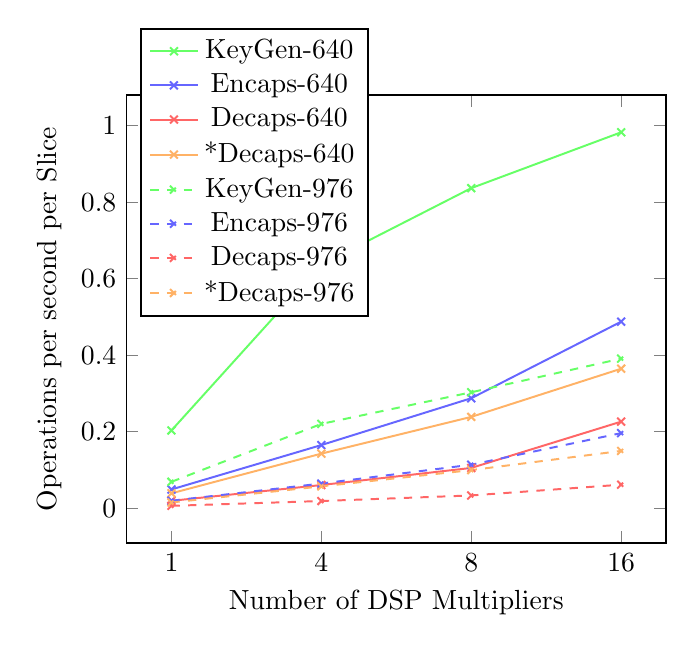
\begin{tikzpicture}
	\begin{axis}[
		xlabel=Number of DSP Multipliers,
		ylabel=Operations per second per Slice,
		line width=0.25mm,
		xtick={0,1,2,3},
		xticklabels={1,4,8,16},
		legend style={at={(0.45,1.15)}}
]
	\addplot[color=green!60,mark=x] coordinates {
		(0,0.203448275862069)	
		(1,0.636619718309859)
		(2,0.836466165413534)
		(3,0.982456140350877)
	};
	\addplot[color=blue!60,mark=x] coordinates {
		(0,0.049152542372881)
		(1,0.165171898355755)
		(2,0.287542087542088)
		(3,0.48758865248227)
	};
	\addplot[color=red!60,mark=x] coordinates {
		(0,0.019434026593931)
		(1,0.060747663551402)
		(2,0.105390835579515)
		(3,0.22636815920398)
	};
	\addplot[color=orange!60,mark=x] coordinates {
		(0,0.039074960127592)
		(1,0.14275092936803)
		(2,0.238767650834403)
		(3,0.364663585002568)
	};
	\addplot[color=green!60,mark=x,dashed] coordinates {
		(0,0.069060773480663)	
		(1,0.220454545454545)
		(2,0.303079416531604)
		(3,0.390969162995595)
	};
	\addplot[color=blue!60,mark=x,dashed] coordinates {
		(0,0.019654088050315)
		(1,0.064604810996564)
		(2,0.113805970149254)
		(3,0.196408529741863)
	};
	\addplot[color=red!60,mark=x,dashed] coordinates {
		(0,0.006319514661274)
		(1,0.018932874354561)
		(2,0.033500501504514)
		(3,0.061623056503603)
	};
	\addplot[color=orange!60,mark=x,dashed] coordinates {
		(0,0.015107913669065)
		(1,0.057241379310345)
		(2,0.09969040247678)
		(3,0.149853085210578)
	};
    \legend{KeyGen-640,Encaps-640,Decaps-640,*Decaps-640,KeyGen-976,Encaps-976,Decaps-976,*Decaps-976}
	\end{axis}
\end{tikzpicture}
}
\caption{Comparison of the throughput performance per FPGA slice on a Xilinx Artix-7.}
 \label{fig:hw_line}
\end{figure}